\chapter{Narrative Tenses: Telling Stories}

\section{Lesson Objectives}
In this chapter, you will learn:
\begin{itemize}
    \item How to use the four past tenses to tell a story
    \item The difference between Past Simple, Continuous, and Perfect
    \item Vocabulary: Watch vs. Look
    \item How to sequence events in the past
\end{itemize}

\section{Reading Context}
\begin{readingbox}[title=Dialogue: A Travel Mishap]
\textbf{Alice:} Why were you late yesterday?\\
\textbf{Bob:} It was a nightmare. I \textbf{was waiting} for the bus when it started to rain.\\
\textbf{Alice:} Oh no. Did you have an umbrella?\\
\textbf{Bob:} No. And I \textbf{had left} my jacket at home. By the time the bus arrived, I \textbf{had been waiting} for 30 minutes and I was soaking wet.\\
\textbf{Alice:} That sounds terrible. What happened next?\\
\textbf{Bob:} The bus was full, so it didn't stop! I \textbf{had to} walk home.
\end{readingbox}

\section{Key Concepts: Watch vs. Look}

\begin{vocabbox}[title=Confusing Verbs]
\begin{itemize}
    \item \textbf{Watch:} For things that move or change (TV, sports, people).
    \begin{itemize}
        \item I \textbf{watch} football on weekends. \trans{Miro fútbol...}
    \end{itemize}
    \item \textbf{Look (at):} For things that are still (pictures, art, objects).
    \begin{itemize}
        \item \textbf{Look at} this photo! \trans{¡Mira esta foto!}
    \end{itemize}
\end{itemize}
\end{vocabbox}

\section{Grammar Focus: Narrative Tenses}

To tell a good story, we use four tenses:

\begin{grammarbox}[title=1. Past Simple]
\textbf{Use for:} Completed actions in the past. The main events of the story.
\begin{itemize}
    \item I \textbf{woke} up and \textbf{got} out of bed.
\end{itemize}
\end{grammarbox}

\begin{grammarbox}[title=2. Past Continuous]
\textbf{Use for:} Actions in progress at a specific time. Setting the scene.
\begin{itemize}
    \item The sun \textbf{was shining} and the birds \textbf{were singing}.
\end{itemize}
\end{grammarbox}

\begin{grammarbox}[title=3. Past Perfect]
\textbf{Use for:} Actions that happened \textbf{before} the main story.
\begin{itemize}
    \item When I arrived, the train \textbf{had left}. (The train left \textit{before} I arrived)
\end{itemize}
\end{grammarbox}

\begin{grammarbox}[title=4. Past Perfect Continuous]
\textbf{Use for:} Actions in progress up to a point in the past. Emphasizes duration.
\begin{itemize}
    \item I \textbf{had been waiting} for 2 hours when he finally arrived.
\end{itemize}
\end{grammarbox}

\section{Visualizing the Tenses}

\begin{center}
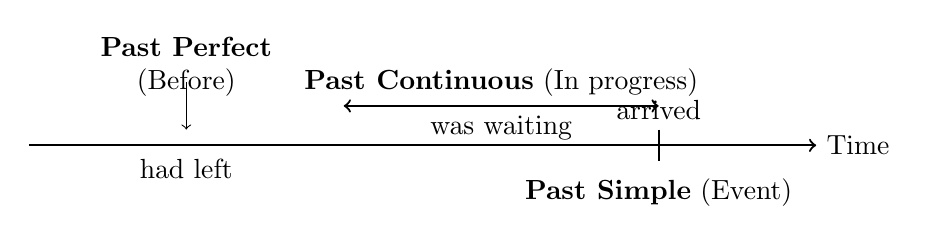
\begin{tikzpicture}
    \draw[->, thick] (0,0) -- (10,0) node[right] {Time};
    
    % Past Perfect
    \node[align=center] at (2,1) {\textbf{Past Perfect}\\(Before)};
    \draw[->] (2,0.8) -- (2,0.2);
    \node at (2,-0.3) {had left};

    % Past Continuous
    \draw[thick, <->] (4,0.5) -- (8,0.5);
    \node[above] at (6,0.5) {\textbf{Past Continuous} (In progress)};
    \node[below] at (6,0.5) {was waiting};

    % Past Simple
    \draw[thick] (8,0.2) -- (8,-0.2);
    \node[below] at (8,-0.3) {\textbf{Past Simple} (Event)};
    \node[above] at (8,0.2) {arrived};
\end{tikzpicture}
\end{center}

\section{Practice Exercises}

\subsection{Exercise 1: Watch or Look?}
Choose the correct verb.

\begin{enumerate}
    \item I like to (watch/look) the sunset.
    \item Can you (watch/look) at this report?
    \item We (watched/looked) a movie last night.
    \item She (watched/looked) at him in surprise.
\end{enumerate}

\subsection{Exercise 2: Choose the Correct Tense}
Select the best option.

\begin{enumerate}
    \item When I arrived, they (finished / had finished) dinner.
    \item It (rained / was raining) when I left the house.
    \item I (was working / had been working) for 3 hours when the computer crashed.
    \item She (opened / was opening) the door and walked in.
\end{enumerate}

\subsection{Exercise 3: Complete the Story}
Put the verbs in brackets into the correct narrative tense.

Last night, I \underline{\hspace{2cm}} (walk) home when I \underline{\hspace{2cm}} (see) a strange light. It \underline{\hspace{2cm}} (shine) brightly. I \underline{\hspace{2cm}} (never / see) anything like it before.

\subsection{Exercise 4: Writing Task}
Write a short story (80-100 words) about a travel experience. Use at least three different past tenses.

\begin{tcolorbox}[colback=white,height=6cm]
% Write your story here...
\end{tcolorbox}

\section{Key Takeaways}
\begin{itemize}
    \item Use \textbf{Past Simple} for the main events (I went, I saw).
    \item Use \textbf{Past Continuous} for background (The sun was shining).
    \item Use \textbf{Past Perfect} for things that happened earlier (I had forgotten my passport).
    \item Remember: Watch (moving) vs. Look at (still).
\end{itemize}

Number 5

You were dancing salsa in the city centre st 2am